\chapter{OpenOCD}
\section{Einleitung}
% TODO: referenz openocd doku
% \ref{bib:OpenOCDDoku}
% TODO: CLI beschreiben / putty
% OpenOCD ist ein ''On-Chip Debugger''.\cite{bib:OpenOCDHome}
% Diese Bezeichnung ist allerdings etwas irreführend.
OpenOCD\cite{bib:OpenOCDHome} bildet den Software Teil von einem Debugger.
Zusammen mit einem Hardware Adapter bildet OpenOCD einen vollständigen Debugger und kann als Ersatz für einen teuren Debugger wie beispielsweise dem BDI 3000 von Abatron verwendet werden.

Der Adapter bildet dabei das elektrische Interface zum Prozessor und muss auch auf den Prozessor abgestimmt sein.
Relevant sind dabei unter anderem der Transport Layer (JTAG/SWD) das elektrische Potential und natürlich auch der Physikalischer Stecker.
In den meisten Fällen basieren solche Adapter, wenn sie zusammen mit OpenOCD verwendet werden, auf dem FT2232 Chip von FTDI.
Solch ein generischer Adapter ist in der Abbildung \ref{fig:GenerischerFT2232Adapter} zu sehen.

\begin{figure}[htbp]
	\centering
		% 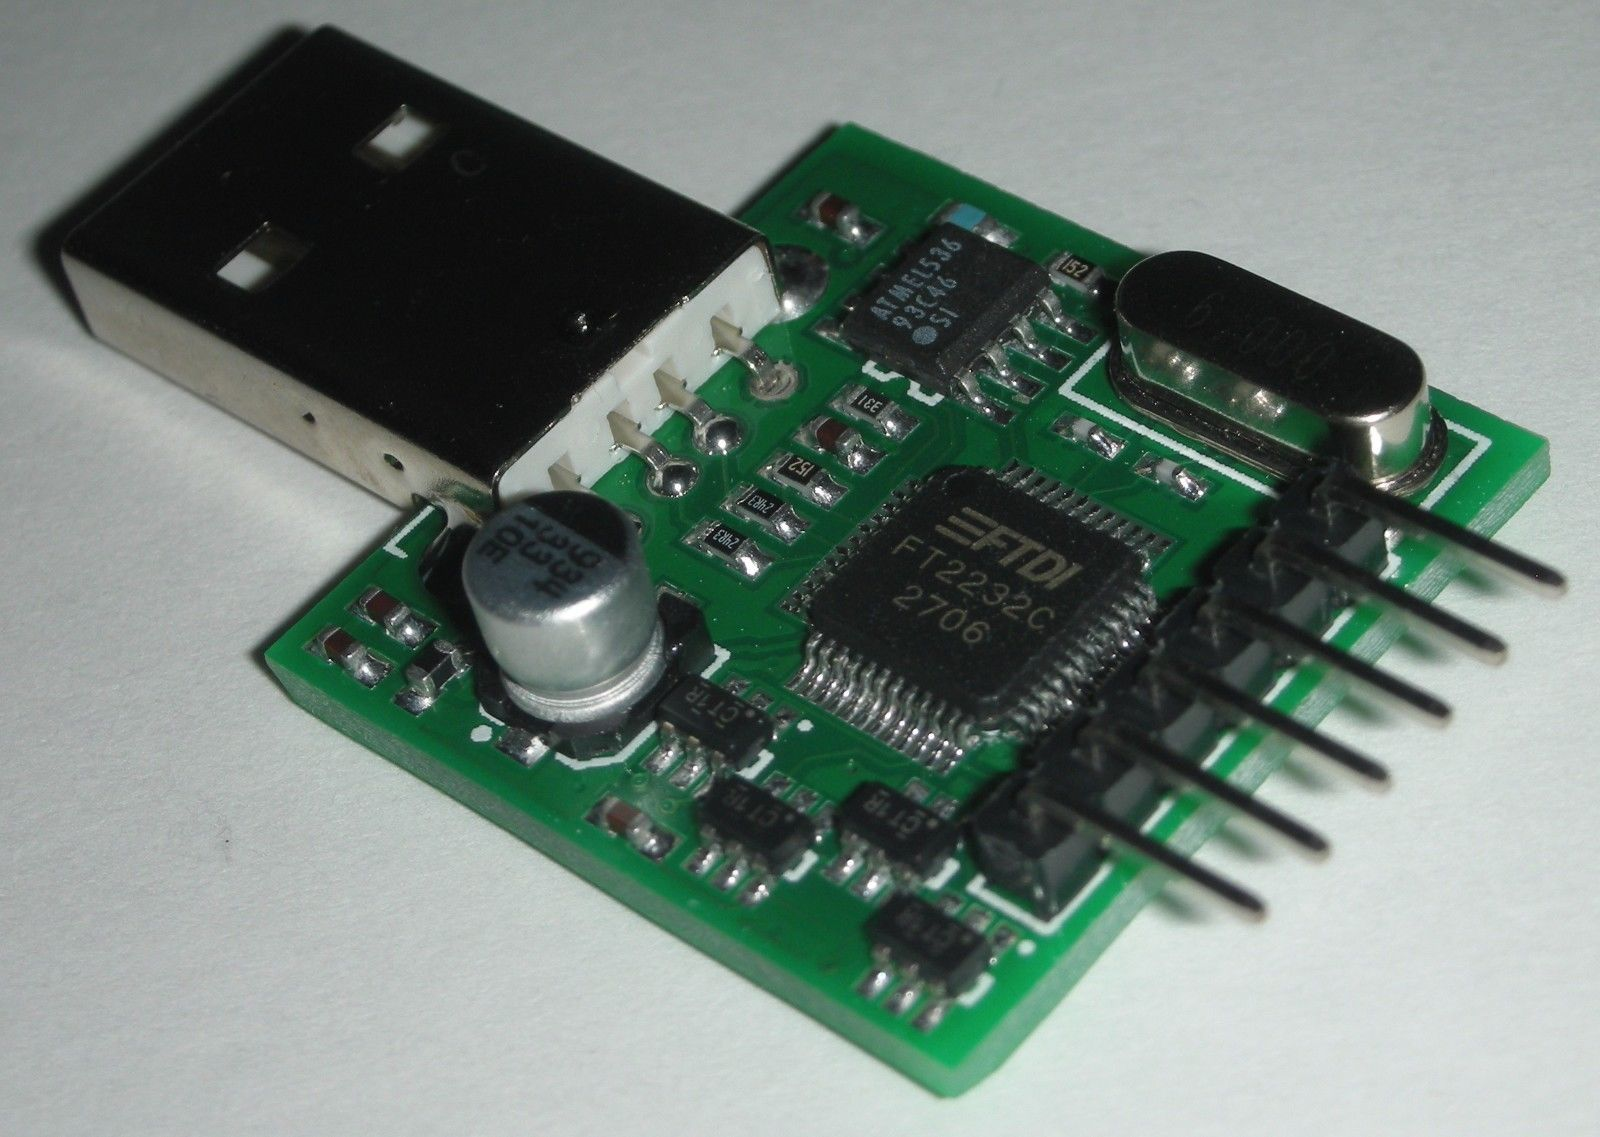
\includegraphics[width=\textwidth,height=\textheight,keepaspectratio]{images/JTAGAdapter.jpg}
		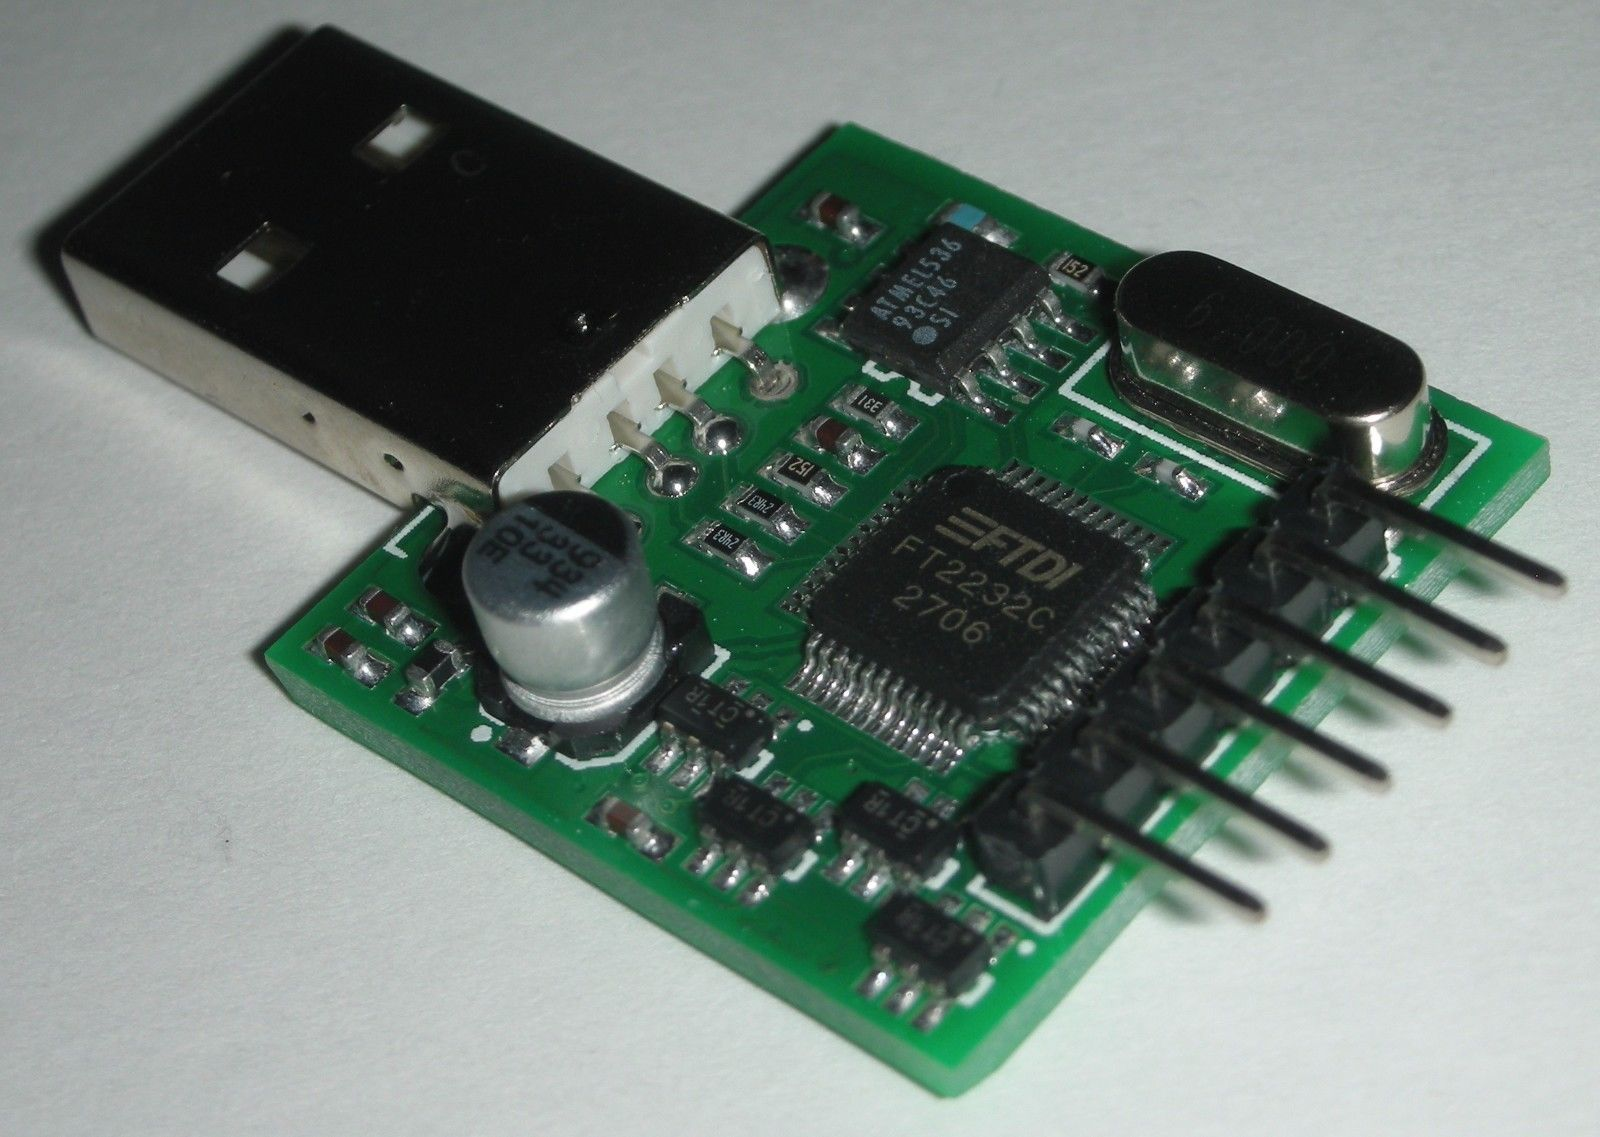
\includegraphics[width=7cm,keepaspectratio]{images/JTAGAdapter.jpg}
	\caption{Generischer JTAG Adapter mit einem FTDI FT2232\cite{bib:ebayJTAGAdapter}}
	\label{fig:GenerischerFT2232Adapter}
\end{figure}

Bei Experimentierboards ist der FT2232 oft auch direkt auf das Board aufgelötet.
So kann eine einfache USB Verbindung genutzt werden, um den Prozessor zu debuggen.
Beim Zybo wurde ebenfalls dieser Ansatz verfolgt.
Aus diesem Grund reicht ein einfaches USB Kabel um den Prozessor auf dem Zybo auf einer Hardware-Ebene debuggen zu können.

\section{Installation}
\subsection{Installation - OpenOCD}
OpenOCD kann direkt vom Sourcecode kompiliert werden\footnote{http://sourceforge.net/p/openocd/code/} oder auch als vorkompiliertes Binary herunter geladen werden.
Für diese Arbeit wurde das vorkompilierte Windows Binary für ARM Cores Version 0.10.0 von folgender URL verwendet:\\
\textit{http://www.freddiechopin.info/en/download/category/4-openocd?download=154\%3Aopenocd-0.10.0}

Das eigentliche Binary befindet sich im Ordner:\\
\texttt{/openocd-0.10.0/bin-x64/} 

Das User Manual befindet sich im Ordner:\\
\texttt{/openocd-0.10.0/} 


\subsection{Installation - USB Driver WinUSB}
Damit OpenOCD mit dem FT2232 Chip kommunizieren kann, werden noch die richtigen USB Treiber benötigt.
Die Installation der Treiber ist am einfachsten mit den \textit{USB Driver Tool}, welches man unter folgender Adresse findet:\\
\textit{http://visualgdb.com/UsbDriverTool/}

Das Zybo muss per USB mit dem PC verbunden sein, damit der Treiber installiert werden kann.
Wenn der Jumper '\textit{J15}' auf USB gesetzt ist, dann wird keine zusätzliche Stromversorgung für das Zybo benötigt.

Öffnet man das \textit{USB Driver Tool} werden alle USB Devices aufgelistet.
Das Device mit der \textit{Vendor ID=0403, Device ID=6010} und \textit{Interface 0} ist das JTAG Interface vom FT2232.
Mit einem Rechtsklick darauf kann man den \textit{Install WinUSB} Treiber auswählen und installieren.
Abbildung \ref{fig:InstallWinUSBDriver} zeigt die Liste mit allen USB Devices und das Kontextmenü für die Installation des richtigen Treibers.
Nachdem das Zybo einmal aus- und wieder einschaltet wird, ist der Treiber einsatzbereit.

Das Device mit der \textit{Vendor ID=0403, Device ID=6010} und \textit{Interface \textbf{1}} ist die UART Verbindung zum Prozessor.
Dieser Treiber darf \textbf{nicht} ersetzt werden.

\begin{figure}[htbp]
	\centering
		% 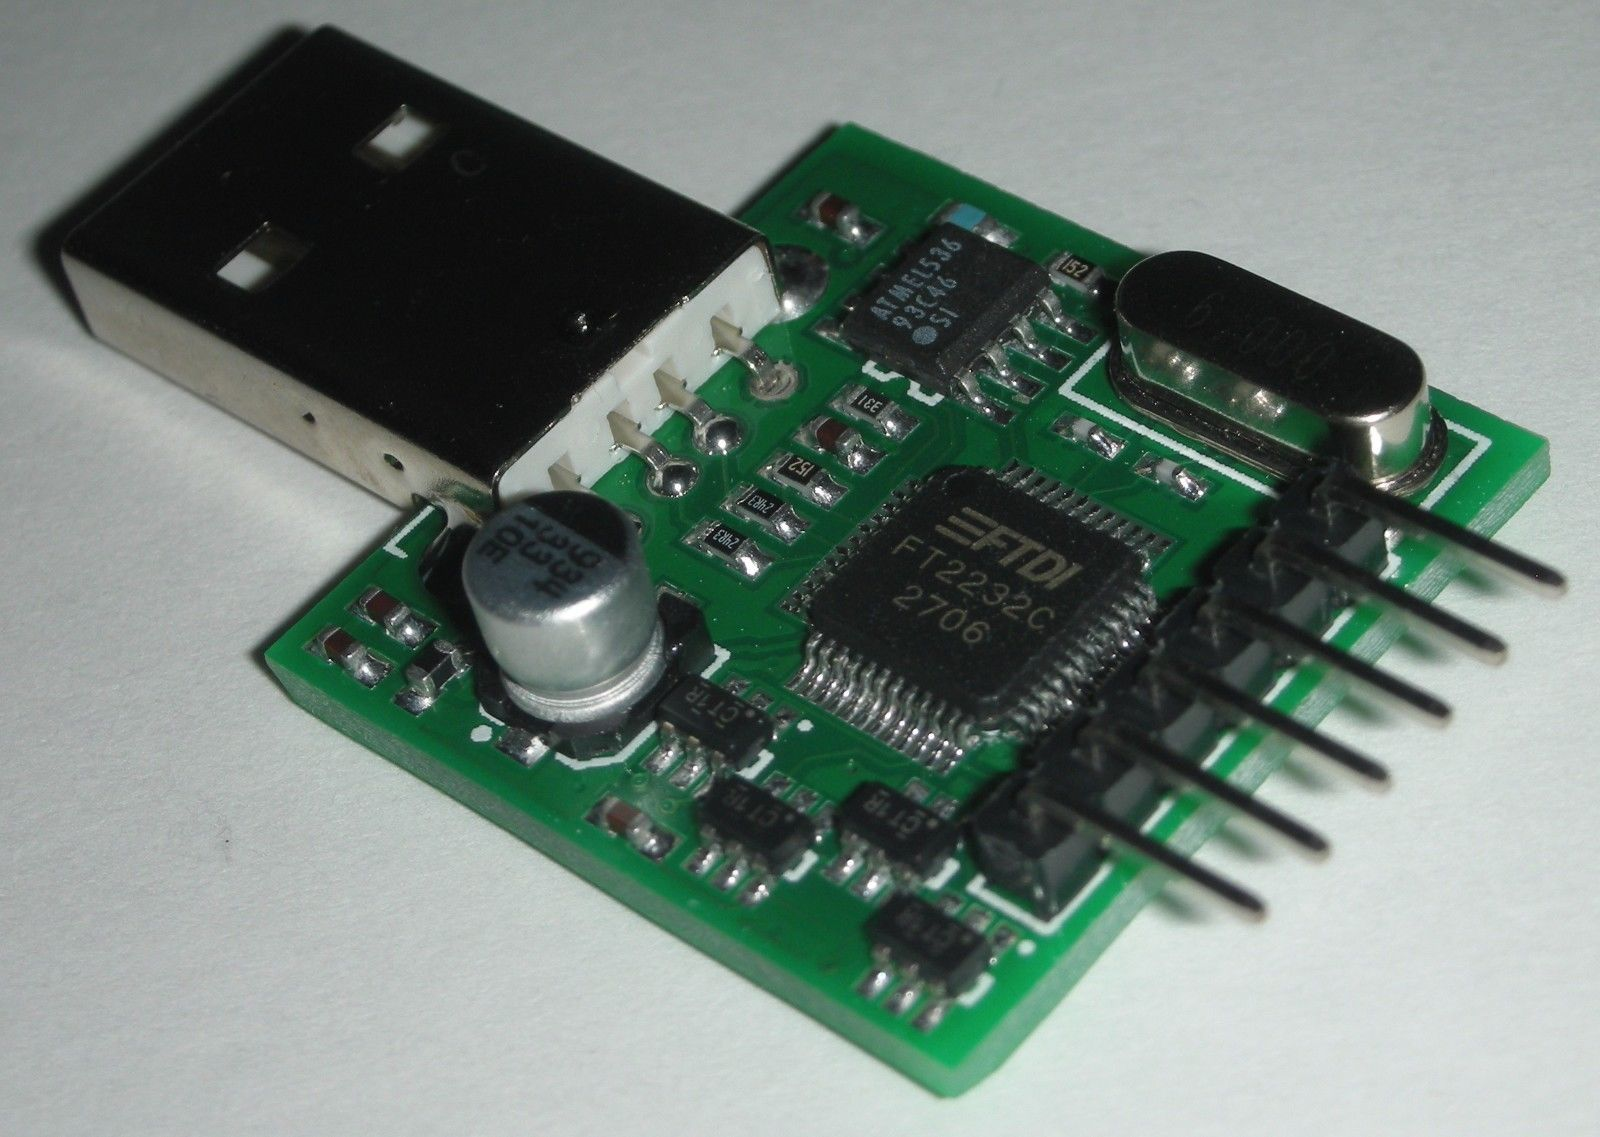
\includegraphics[width=\textwidth,height=\textheight,keepaspectratio]{images/JTAGAdapter.jpg}
		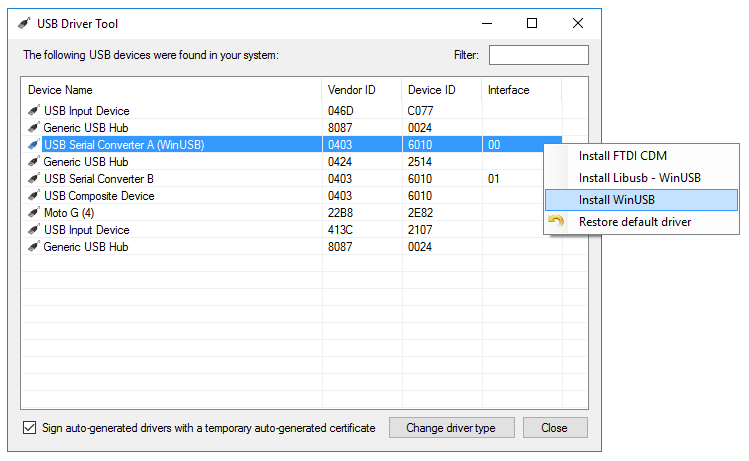
\includegraphics[width=12cm,keepaspectratio]{images/InstallWinUSBDriver.png}
	\caption{Installation des \textit{WinUSB} Treibers mit dem \textit{USB Driver Tool}}
	\label{fig:InstallWinUSBDriver}
\end{figure}


\section{OpenOCD Konfiguration}
% TODO: zum starten siehe kapitel ...
% TODO: Files anhängen
% nicht einfach
% spezielle sprache jim-tcl
OpenOCD unterstützt eine Vielzahl von Adaptern und Targets (Prozessoren).
Beim Start muss die Software für die verwendete Hardware konfiguriert werden.
Die Konfiguration erfolgt mit Konfigurationsscripts (*.cfg) in der Scriptsprache \textit{Jim-Tcl}.
\textit{Jim-Tcl} ist eine abgespeckte Version von \textit{Tcl}\footnote{http://www.tcl.tk}.

Normalerweise werden die Scripts in die drei Gruppen \textit{interface, board} und \textit{target} aufgeteilt.
So kann einfach ein Script ausgewechselt werden, wenn man den gleichen Adapter aber einen anderen Prozessor verwenden will.
Im Pfad \textit{openocd-0.10.0/scripts} befinden sich eine Sammlung von Konfigurationsscripts für Standardhardware.

Mit folgendem Befehl kann OpenOCD mit Konfigurationsscripten nach Wahl gestartet werden:\\
\texttt{openocd -f script1.cfg -f script2.cfg -f script3.cfg}


\section{OpenOCD Konfiguration - Interface}
Die Interface Konfiguration beschreibt hauptsächlich den verwendeten Adapter.
Da beim Zybo kein Adapter verwendet wird, sondern der aufgelötete FT2232, wird mit diesem Script der FTDI Chip und dessen Anbindung an den Zynq konfiguriert.

Da ein FTDI-Chip als Interface verwendet wird, sollte ein passender Script unter \textit{openocd-0.10.0/scripts/interface/ftdi/} zu finden sein.
Keiner der Scripts passt von Namen her auf \textit{Zynq, Zybo} oder \textit{FT2232}.
Eine Google Suche nach einem passenden Script war erfolgreicher.
Ein Github User mit dem Namen \textit{emard} hat folgenden Script in einem von seinen Repositories gespeichert:

% TODO neutrale text-farben
\textit{ftdi-zybo.ocd:}
\begin{lstlisting}
#
# ZYBO ft2232hq usbserial jtag
#

interface ftdi
ftdi_device_desc "Digilent Adept USB Device"
ftdi_vid_pid 0x0403 0x6010

ftdi_layout_init 0x3088 0x1f8b
#ftdi_layout_signal nTRST -data 0x1000 -oe 0x1000
# 0x2000 is reset
ftdi_layout_signal nSRST -data 0x3000 -oe 0x1000
# green MIO7 LED
ftdi_layout_signal LED -data 0x0010
#ftdi_layout_signal LED -data 0x1000

reset_config srst_pulls_trst

\end{lstlisting}

Zeile 5 bis 7 konfigurieren das Interface als ein standard-FTDI Interface.
Von OpenOCD werden neben dem FT2232 auch noch andere Chips unterstützt.
Zeile 7 definiert die Vendor und Device-ID des USB Devices.

\subsection{Resetverhalten}
Liest man aus einer unerlaubten Speicheradresse (\texttt{CLI: mdw 0x40000000}), dann hängt sich die Debug-Peripherie im Zynq auf.
Nach so einem unerlaubten Speicherzugriff können auch keine erlaubten Speicherstellen mehr gelesen werden.
Beim Versuch erscheint die Fehlermeldung:\\
 \texttt{Timeout waiting for cortex\_a\_exec\_optcode}.\\
Mit einem manuellen Powercycle vom Zybo kann die Hardware wieder zurückgesetzt werden.

Mit OpenOCD ist es grundsätzlich auch möglich, einen Reset automatisch durchzuführen.
Dabei wird zwischen einen \textit{System Reset} (SRST) und dem \textit{TAP Reset} (TRST) unterschieden.
Der SRST führt dabei einen Powercycle vom ganzen System durch, der TRST setzt nur den TAP zurück

% TODO: warum memory location nicht erlaubt
Beim obigen Script ist aber das Resetverhalten nicht sauber definiert.
Mit dem Befehl \texttt{''CLI: reset halt''} im CLI sollte ein Reset vom FT2232 durchgeführt werden.
Der Befehl führt aber zur Fehlermeldung:\\
\texttt{... zynq.cpu0: how to reset? ...}

In der OpenOCD Dokumentation\cite{bib:OpenOCDDoku} im Kapitel \textit{9 Reset Configuration} ist beschrieben, wie das Resetverhalten konfiguriert werden kann.
Mit dem Script-Befehl \texttt{''reset\_config srst\_only''} wird der TAP Reset ignoriert.
So kann das Problem auf den System Reset begrenzt werden.

Wenn OpenOCD mit der neuen Konfiguration neu gestartet wird, dann scheint der Befehl \texttt{''CLI: reset halt''} zu funktionieren.
Greift man vorher aber wieder auf eine ungültige Speicherstelle zu, dann erscheint beim Reset die Fehlermeldung\\
\texttt{... Timeout waiting for dpm prepare ...}.\\
Das legt die Vermutung nahe, dass der Zynq nicht ordentlich zurück gesetzt wurde.

Zeile 12 (\texttt{ftdi\_layout\_signal nSRST -data 0x3000 -oe 0x1000}) konfiguriert die I/O Pins des FT2232 welche für den System Reset verwendet werden.
Auf dem elektrischen Schema vom Zybo\ref{anhang:schemaZybo} könnte man überprüfen, welche I/Os vom FT2232 effektiv für den Reset verwendet werden.
Die Seite mit dem Schema für den FT2232, Seite 7, ist aber als einzige Seite im Schema nicht veröffentlicht worden.
Die korrekten I/O Pins lassen sich also nicht mit dem Schema ermitteln.

% ftdi_layout_signal nSRST -data 0x3000 -oe 0x1000

% \ref{bib:OpenOCDDoku}

% 


% TODO änderungen für reset


\section{OpenOCD Konfiguration - Board}
Da beim Zybo der Adapter direkt auf dem Board ist, ist die Bordkonfiguration bereits im Konfigurationsscript für das Interface enthalten.

\section{OpenOCD Konfiguration - Target}
Für das Target, in diesem Fall der Zynq 7000 SOC, ist bereits ein Script unter \textit{openocd-0.10.0/scripts/target/zynq\_7000.cfg} enthalten.
In diesem Script werden nicht nur beide Kerne des Prozessors definiert, sondern auch ein TAP\footnote{Test Access Port} für den FPGA Teil.
Es ist also auch möglich, den FPGA mit dieser Toolchain zu laden.
% zynq_7000.cfg